\chapter{Working with magnetic resonance images of the brain}
\label{chp:chp2}

\section{Human brain anatomy}
\label{sec:chp2:anatomy}
\index{brain anatomy}

The human brain consists of multiple structures including the large
cerebrum, the smaller cerebellum, and the brain stem. These structures
can easily be identified from MR images of the
brain (Figure \ref{fig:chp2:brain}). The cerebrum is composed of the
left and right hemispheres, which are connected through bundles of
nerve fibers (the corpus callosum).

\index{brain anatomy!white matter}
\index{brain anatomy!gray matter}

There are two main types of brain cells: neurons (or nerve cells) and
glial cells. Each neuron is generally composed of a cell body
(\emph{soma}), a long nerve fiber (\emph{axon}), and other
branching extensions (\emph{dendrites}). The spatial distribution
of the brain cells results in two primary types of brain tissue
matter: white and gray matter\footnote{Neurons, roughly speaking, have
  a cell body (soma) and branches (axons and dendrites) that extend
  from the cell body.  Axons are either covered with a lipid-rich
  (fatty) layer called myelin (myelinated axons) or 
  surrounded by other cells (unmyelinated axons); myelin helps the
  axons conduct electrical signals over long distances. Myelin, being
  fatty, gives off a white-ish color; conversely, unmyelinated axons,
  dendrites, and neural cell bodies, in close proximity to
  microcirculation, appear gray.  This is the origin of the terms
  \textit{gray matter} and \textit{white matter}.}. White matter mainly consists of
bundles of (myelinated) axons while gray matter includes neuronal cell
bodies, and glial cells. The distribution of white and gray matter in
the cerebrum is shown in Figure~\ref{fig:chp2:brain} (right), which
demonstrates the white matter and the cortical and sub-cortical gray
matter. The sub-cortical gray matter includes a number of important
structures or regions located deep inside the brain, such as~the
hippocampus, basal ganglia and thalamus.
\begin{figure}[t]
  \centering
  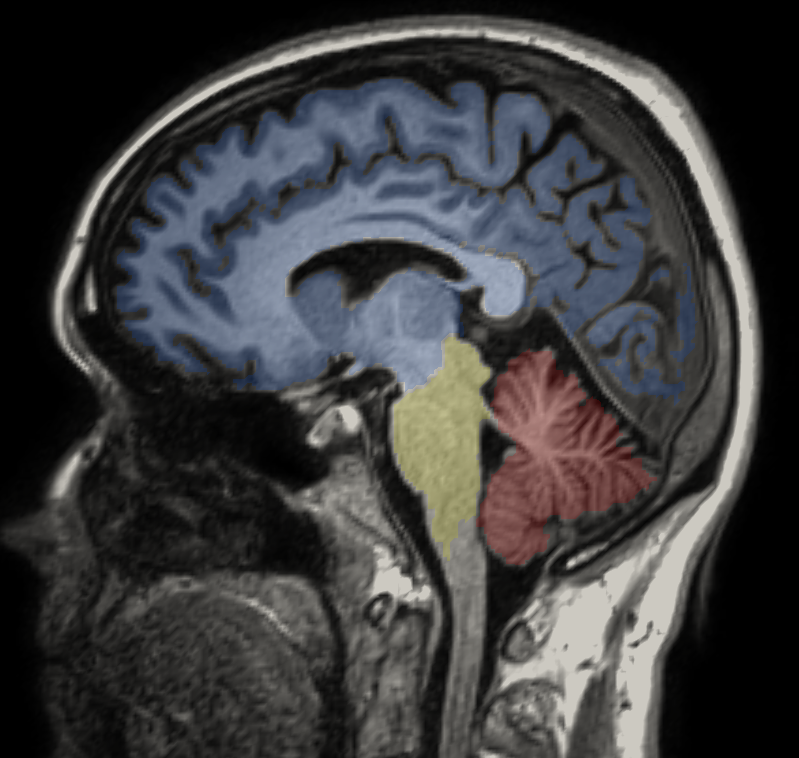
\includegraphics[width=0.48\textwidth]{./graphics/chp2/exp-brain.png}
  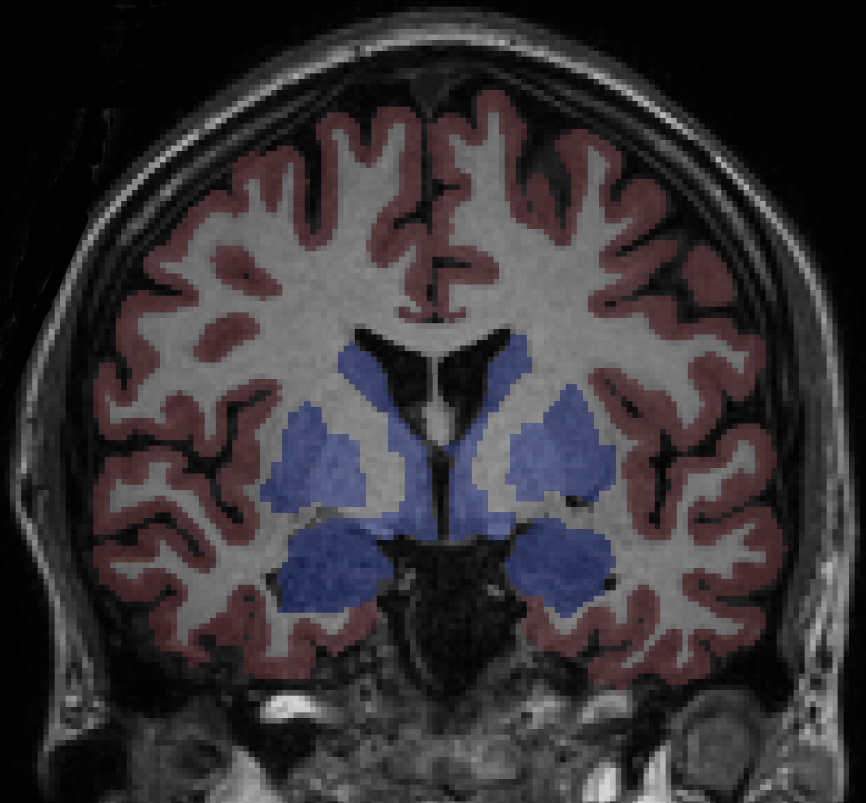
\includegraphics[width=0.48\textwidth]{./graphics/chp2/exp-matters.png}
  \caption{MR images (T1-weighted) of the human brain. Left: A sagittal
    (longitudinal) cross-section of the human brain with the cerebrum
    in blue, the cerebellum in red, and the brain stem in yellow. Right: A coronal
    slice of the brain. The tissue matter
    composition of the cerebrum is marked by color with red denoting
    the cortical gray matter, blue denoting the subcortical gray matter
    and white denoting the white matter. (The colors have been added after
    post-processing.)}
  \label{fig:chp2:brain}
\end{figure}

\index{brain anatomy!meninges} \index{brain anatomy!ventricles} The
brain is enclosed and protected by three layers of meninges; the
outermost \emph{dura}, the middle \emph{arachnoid} and the innermost
\emph{pia} membrane. The narrow space between the pial and arachnoid
membranes is filled with cerebrospinal fluid (CSF) and is referred to
as the \emph{subarachnoid space} (SAS). The SAS extends around the
brain and further down along the spinal cord. The SAS is also
connected to the ventricular system, a system of interconnected CSF
compartments surrounded by the brain. The ventricular system consists
of the two lateral ventricles and the third and fourth ventricles,
shown in Figure~\ref{fig:chp2:ventricles}. The thin passage between
the third and fourth ventricle is known as the cerebral aqueduct.
\begin{figure}
  \centering
  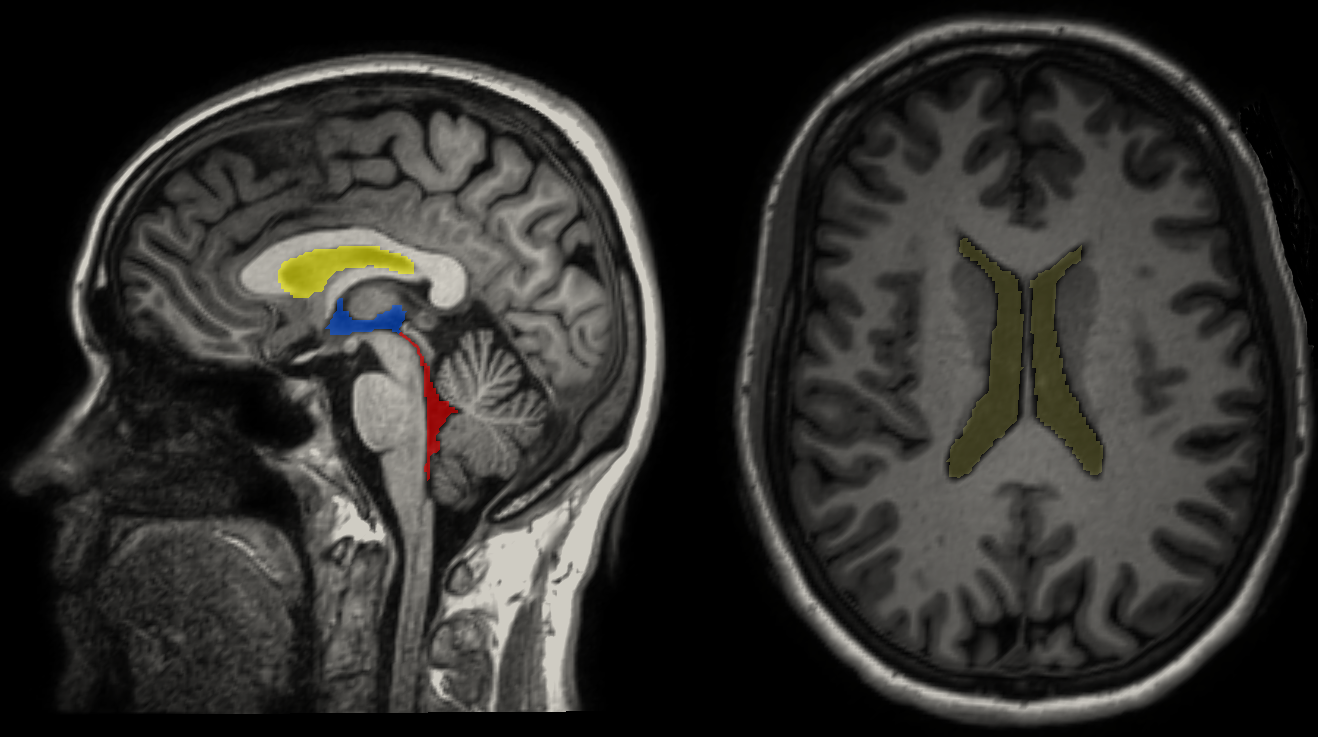
\includegraphics[width=0.98\textwidth]{./graphics/chp2/exp-vent.png}
  \caption{Sagittal (left) and axial (right) MR image cross sections
    of the brain with the lateral ventricles marked in yellow, the 3rd
    ventricle marked in blue and the 4th ventricle and the aqueduct
    marked in red. The white region surrounding the lateral
    ventricles, on the left, is the corpus callosum. The distinction
    between (cortical) gray and white matter is also clearly visible
    on the right.}
  \label{fig:chp2:ventricles}
\end{figure}

We refer the reader, for example, to \cite{gray2009gray} for a good
introduction to human brain anatomy and \cite{boron2016medical} for a
general introduction to human physiology.

\section{Magnetic resonance imaging}

\index{MRI}
\index{MRI!sequence}
Magnetic resonance imaging (MRI) is a rich and versatile technique for
the non-invasive medical imaging of the brain and other organs.  The method has 
its roots in studies of Isidor Rabi; dating to the early 20th century.  Rabi 
was able to ascertain information on the rotation and magnetic movements of 
the nuclei of atoms and molecules \cite{thomas2013}.  MRI leverages these types 
of magnetic properties; specifically for the nucleus of elemental hydrogen, 
which is abundant in tissues and in fat \cite{berger2002}.  An MRI scanner 
creates a strong magnetic field, aligning the poles of hydrogen atoms along the 
MRI scanner's axis.  A radio wave is added to the magnetic field, causing the 
hydrogen nuclei to resonate, and different (scanner) slices of the body resonate 
differently.  Turning off the applied radio frequency induces the realignment 
of the hydrogen nuclei with the applied magnetic field which; this process, in 
turn, causes the emission of another radio wave signal which the MRI scanner 
measures.  The intensity of this last signal is what we visualize as MRI 
images \cite{berger2002}.    


The MRI method can be used for detailed investigations of tissue morphology and
structure (structural MRI), tissue properties (e.g.~diffusion weighted MRI),
blood flow (perfusion MRI) as well as aspects relating to brain
function (functional MRI). As detailed above, an MR image is constructed from 
the interaction of a strong magnetic field and radio waves.  The specifics of 
the procedure can be controlled by manipulating factors that affect this 
interaction; one such factor is the magnetic field gradient.  A specific set of 
changing magnetic gradients is referred to as an MRI \emph{sequence}, which in 
turn has a number of parameters. We briefly describe a few key MRI sequences 
here; the interested reader can find more information in
e.g.~\cite{haacke1999magnetic, payne2017cerebral, alexander2007diffusion}.

\subsection{Structural MRI: T1- and T2-weighted images}
\label{sec:T1T2}

\index{MRI!T1}
\index{MRI!T2}
Structural MRI provides high resolution images of brain anatomy and
can thus give information about the shape, size and composition of
different brain compartments and regions\footnote{gray matter (cortical) and 
white matter regions are defined vis-a-vis a segmentation and 
parcellation process.  Parcellations are discussed in more detail in 
Chapter~\ref{sec:chp4:tools:remove-vent:extraction}}. 

Examples of structural MRI
sequences include T1- and T2-weighted images, as already
encountered in Figures~\ref{fig:chp2:brain} and
\ref{fig:chp2:ventricles}. Such images are well suited for defining
brain geometry models and will be used extensively for this purpose
(Chapters~\ref{chp:chp3}--\ref{chp:chp4}). A brief introduction to T1-
and T2-weighted images can be found in~\cite{pooley2005fundamental}.

T1- and T2-weighted images correspond to different (groups of) MRI
sequences, each with their own parameters and characteristics. A T1-
or T2-weighted image is a three-dimensional image, typically viewed as
a stack of black-and-white images of different planes (axial, coronal
or sagittal) of the brain. The colored shading is referred to as the
\emph{signal intensity} with white representing a high signal
intensity and black representing low intensity (with gray tones
representing intermediate values). Both imaging sequences (T1- and
T2-weighted) produce different signal intensities for different types of
tissue and fluids, but the two differ in their dominant intensities.

\begin{figure}
  \centering
  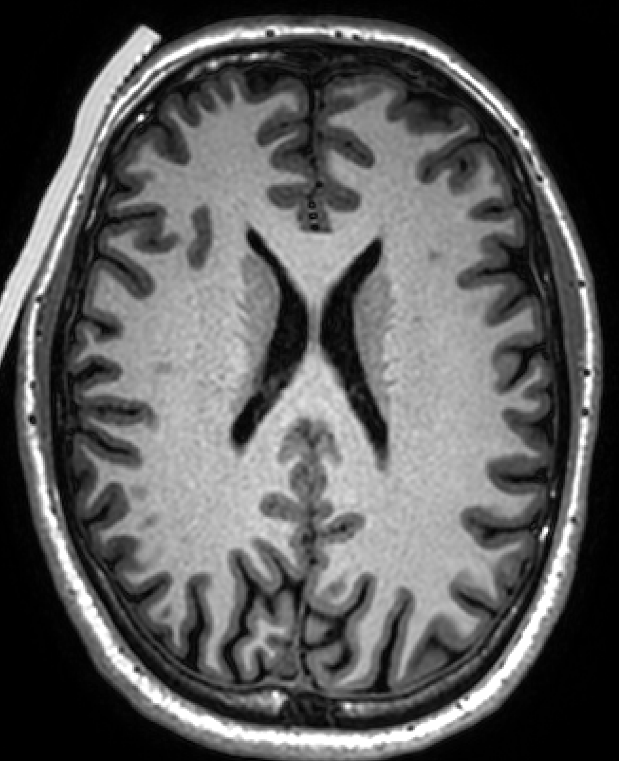
\includegraphics[width=0.415\textwidth]{./graphics/chp2/T1-image.png}
  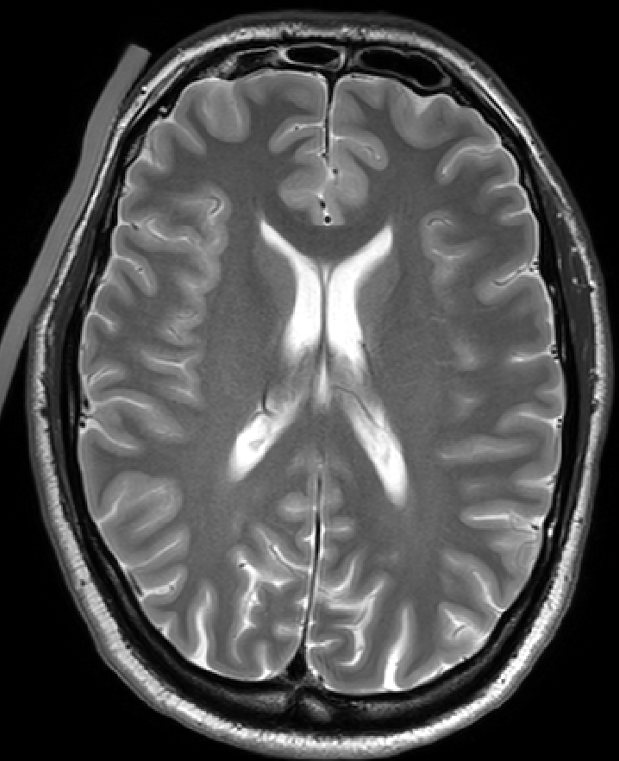
\includegraphics[width=0.415\textwidth]{./graphics/chp2/T2-image.png}
  \caption{T1-weighted image (left) versus T2-weighted image (right).
    In the T1-weighted image, white matter is recognized as light
    gray, whereas the darker gray lining the surface of the brain is
    gray matter. T1-weighted images are used particularly because they
    exhibit a sharp contrast between gray and white matter.  The
    T2-weighted image shows the CSF as almost white and provides good
    contrast between the CSF and the brain, but less contrast between
    white and gray matter. Note also that blood is dark in
    T2-weighted images.}
  \label{fig:chp2:t1vt2}
\end{figure}
In T1-weighted images, fat gives off a high intensity signal and
appears white, while fluids give off a low intensity signal and appear
black. Therefore, the brain tissue appears as different shades of gray
with white matter appearing lighter than gray matter
(Figure~\ref{fig:chp2:t1vt2} (left)). T1-weighted images are effective
at differentiating between white and gray matter, but less effective
at distinguishing between, for example, the CSF (black) and the gray
matter (dark gray). In particular, it can be difficult to identify
fluid compartments such as the ventricles, the aqueduct, and SAS from
T1-weighted images alone.

%
\index{brain anatomy!ventricles}
%
In T2-weighted images on the other hand, fluids give off a high
intensity signal and appear white (Figure~\ref{fig:chp2:t1vt2}
(right)). Such images are less effective at distinguishing between
white and gray matter, but can provide good contrast between the CSF
(white) and brain matter (gray). T2-weighted images can thus
supplement data from T1-weighted images for identifying and separating
the ventricles and aqueduct from subcortical gray matter.

\subsection{Diffusion weighted imaging and diffusion tensor imaging}

\begin{figure}
  \sidecaption
  \centering
  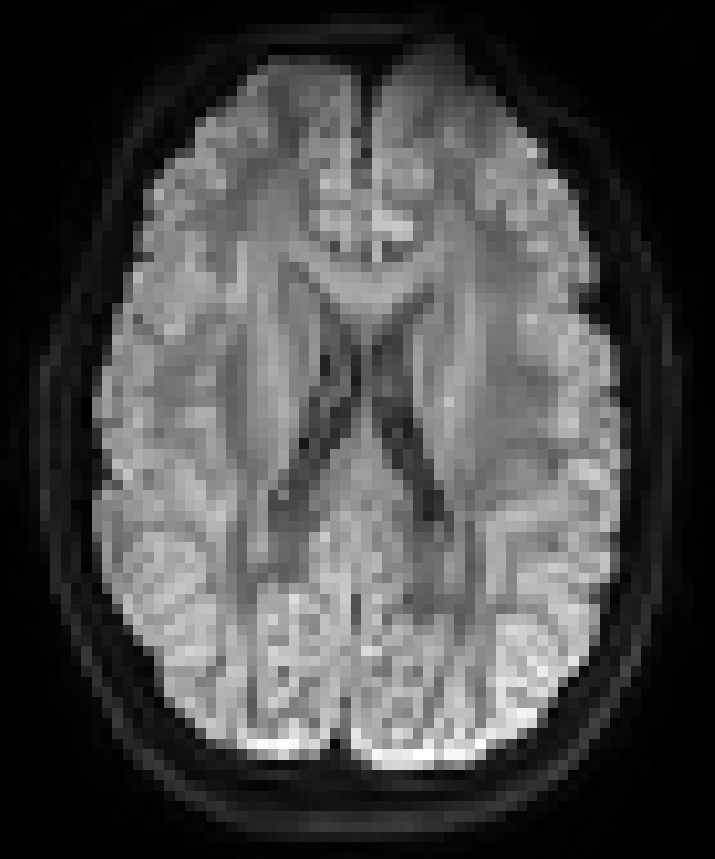
\includegraphics[width=0.49\textwidth]{./graphics/chp2/DTI-slice-image-crop.png}
%\caption{A raw, axially-oriented dMRI image of the brain. The ventricles (center) 
%appear in low contrast whereas areas of high diffusion bias, along axonal fibers, 
%are more pronounced.}
\caption{A raw, axially-oriented dMRI image of the brain. Notice that the 
ventricles (center) appear in lower contrast due to the strongly isotropic 
diffusion of the water contained within them.} 
\label{fig:chp2:dti}
\end{figure}

%
\index{DTI}
%
Diffusion MRI (dMRI) is an imaging modality that detects water
molecule movement patterns \cite{jeurissen2017,soares2013hitchhiker}.
Both isotropic and anisotropic diffusion coefficients can be
determined.  Diffusion tensor imaging (DTI) is a specific type of 
diffusion-weighted MRI. Figure~\ref{fig:chp2:dti}, an example of a 
DTI-weighted image.  At a high level, a reference image (of T2 type) 
is used as a comparison and the DTI imaging process measures the 
difference in that reference signal with several follow-up signals.  The 
resulting sequence provides information about how water diffuses in different 
regions of the brain.
%high signal intensities (white regions of the image) correspond
%to areas where the diffusive motion of particles has a coherent
%directionality; conversely, low directionality regions, where the
%diffusive behavior is relatively undirected (i.e.~more isotropic),
%correspond to a low (darker) intensity. For instance, in the
%ventricles, which are filled with CSF, the molecular
%motion is less restricted and molecules can move about in almost any
%direction; these regions are therefore darker.  Along axonal
%bundles, which heavily bias the extracellular fluid flow, we see
%higher signal intensities and these regions of a dMRI image appear
%brighter.

More specifically, DTI provides information on both the magnitude and 
(multiple) directions of the movement of molecular water in the brain; that is, 
how water travels.  In mathematical terms, DTI provides information regarding 
the diffusion tensor, $D$, in \eqref{eq:diffusion}.  In three dimensions, this 
tensor has nine entries and a global representation given by
\begin{equation}
D = \begin{pmatrix}
  d_{11} & d_{12} & d_{13} \\
  d_{21} & d_{22} & d_{23} \\
  d_{31} & d_{32} & d_{33}
\end{pmatrix}.
\end{equation}
Each of the entries $d_{ij}$ can be a function of the position $x \in
\R^3$. We will extract the heterogeneous, anisotropic,
and patient-specific diffusion tensor from DTI 
image data in Chapter~\ref{chap:dti}.  DTI has been used extensively to 
study the layout of brain's white matter tracts; these tracts heavily bias 
the movement of water within the brain. We refer the interested reader to
\cite{jeurissen2017}, and the many sources therein, for a discussion
on more the advanced topics related to the field of dMRI techniques.

\section{Viewing and working with MRI data sets}
\label{sec:chp2:tools:viewers}

\subsection{The DICOM file format}
\index{DICOM}

Medical images, including T1, T2 and DTI, are often stored in the
DICOM file format. DICOM stands for \emph{Digital Imaging and
  Communications in Medicine} and is an imaging
standard~\cite{mildenberger2002introduction}. The format stores both
the image itself and a comprehensive set of meta-data, such as
the imaging protocol and patient identification, which enables
consistent and safe usage across different vendors and software
packages.  

The DICOM format gives the output from an MRI scan as a collection of
files arranged in sequences. A given file within a sequence\footnote{Formally, 
the term \textit{MRI sequence} does not refer to an ordered measure (such as a 
sequence in time) but, rather, to a specific type of pulse sequence, or field 
gradient, that determines the specific imaging protocol.  A T1 
\textit{MRI sequence} produces T1 images, a T2 \textit{MRI sequence} produces 
T2 images, and so forth.  Here, when we speak of `a sequence of files' we are 
referring to the order in which the files are produced by the MRI scanner; this 
is typically reflected in the naming of the files such that IM\_0001 would be 
produced before IM\_0002, and so on.} also contains the necessary information 
to inform the viewer what the next (or previous) file in that file sequence is. 
DICOM files are sometimes stored in a binary file named \emp{DICOMDIR} that 
indexes the entire structure of an MRI dataset. 

\subsection{Working with the contents of an MRI dataset}
\label{sec:chp2:viewmri}
\index{DicomBrowser}

A DICOM viewer is an essential component for viewing and working with
DICOM files. A number of DICOM browsers exist, and we will use
DicomBrowser~\cite{dicombrowser}.  Currently, DicomBrowser is
available\footnote{https://wiki.xnat.org/xnat-tools/dicombrowser} as a
pre-packaged binary download for several operating systems; the source
code\footnote{https://bitbucket.org/xnatdcm/dicombrowser/src/master/}
is also available. On Ubuntu Linux, DicomBrowser comes pre-packaged
as a Debian package file; this type of file can be installed on
Ubuntu using the command \ubuntu{\$ sudo apt install
  /path to file/my-dicombrowser.deb}
\noindent where you should change `path to file' to the path where the  
DicomBrowser installation file (ending in .deb) has been downloaded and change 
the text of `\emp{my-dicombrowser.deb}' to be the specific filename of the 
DicomBrowser installer package. 
%the path to the DicomBrowser package that you downloaded.

We now demonstrate how to extract sequences from an MRI dataset. This
process begins by launching the DicomBrowser utility with the 
command: 
\terminal{\$ DicomBrowser \&}
\noindent After the DicomBrowser window opens, select
\button{File$\rightarrow$Open} from the top menu bar; a dialogue box
will appear with the heading \button{Select DICOM files}. Navigate to
the directory containing the (example) book data set and select the directory
titled \emp{\erniedicom}.  In this directory select the file titled
\emp{DICOMDIR}. The main DicomBrowser window should now show a list of
the patients whose data are included in this dataset (in this case
just one patient).  In the main window (c.f.~Figure~%
\ref{fig:chp2:dicombrwsr-scr} (left)), click the patient, whose ID starts with 
1.3.46, and then click the symbol to the left of the patient ID to expand the 
entry.

\begin{figure}[h]
  \centering
  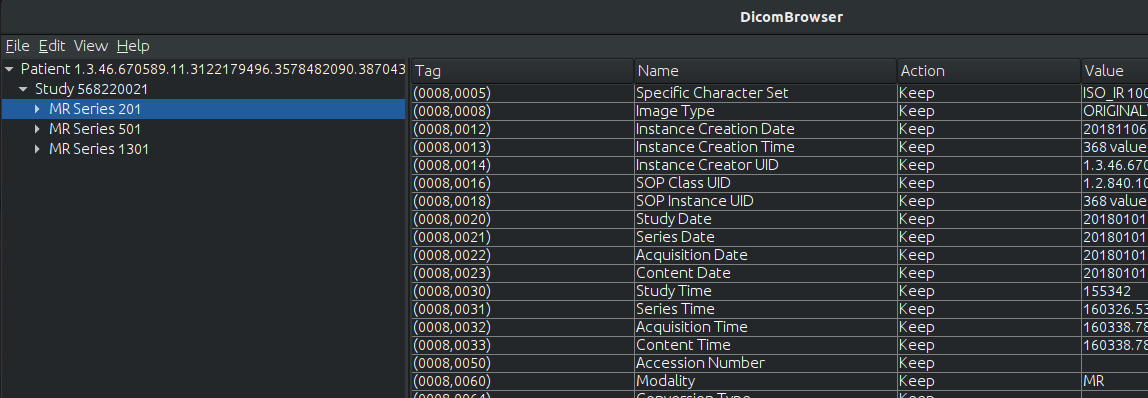
\includegraphics[width=\textwidth]{./graphics/chp2/dicombrowser-d-ext}
  \caption{Example of the DicomBrowser layout and selection of an MR series (\emp{\erniedicom}).} 
  \label{fig:chp2:dicombrwsr-scr}
\end{figure}

A list of studies now appears under the patient ID; generally, a
patient can have several associated studies but the (example) book dataset
contains one study per patient. Expand the study (beginning with 568)
by clicking the symbol to the left. A list of MR series now fills the
main window; many MR series can be contained in a single study and we
see that the \emp{\erniedicom} data contains three series (201, 501 and 1301), 
see Figure~\ref{fig:chp2:dicombrwsr-scr}.

Find MR Series 201 and left-click on it. The secondary window now
contains a list of tags; each tag has an associated name, action, and
value (Figure \ref{fig:chp2:dicombrwsr-scr}). Note that tag (0018,
1030)\footnote{Tag identifiers are not standard, and can differ based
  on the MRI scanner manufacturer.  Generally, we identify a
  sequence from the Name field by looking for a label containing T1,
  T2, or DTI.} is named `protocol name' and has value T13D; this
indicates that MR Series 201 corresponds to a T1-weighted image
sequence. With `MR Series 201' as the current selection, in the DicomBrowser 
(left) window, we can select \button{File$\rightarrow$Save} to extract the 
series; a window then appears which provides extraction options.  We would 
like to extract this series to a directory with a memorable name; we can 
do this by changing `-anon' to `-T13D' to signify that the series we are 
extracting represents a T1 weighted image in 3D.  %
%
%Extract MR Series 201 by clicking
%\button{File$\rightarrow$Save} and change -anon to -T13D. 
We also remark that DicomBrowser can be used to anonymize the data, as
indicated by the default extension {-anon}, or, in general, to change
DICOM tag values either through the GUI or in scripts. 

We can use the same procedure to extract other image sequences. In our
book DICOM images, MR Series 501 is a DTI sequence and MR Series 1301
includes T2-weighted images.  We have already extracted all three series, 
present in the sample \emp{DICOMDIR}, into the (example) book dataset.  Image series 
201 has been extracted to \emp{\erniedicom/T13D}, image series 1301 has been 
extracted to \emp{\erniedicom/T23D} and image series 501 has been extracted to    
\emp{\erniedicom/DTI}.  We note that \emp{\erniedicom/DTI} also contains 
some non-image files; these files are not in the \emp{DICOMDIR} data but 
will be generated, and discussed, in Chapter~\ref{chap:dti}   
%
%We have extracted 501 to the directory
%\emp{DTI} and 1301 to the directory \emp{T23D} in the book dataset.


\section{From images to simulation: A software ecosystem}
\label{sec:chp2:software-ecosystem}
In this section, we provide a brief overview of the software tools that 
comprise the pipeline used in this book. We will extract data from clinical
images, segment the data, extract and work with diffusion tensor
information, generate a finite element mesh, and bring all of this
together to solve a partial differential equation. Along
the way, we will need additional tools for miscellaneous
objectives such as file conversion and visualization. A visual
representation of the patient-specific pipeline from MRI-images to
finite element simulations is shown in Figure
\ref{fig:chp2:imaging-pipeine-overview}.

\begin{figure}
\centering
 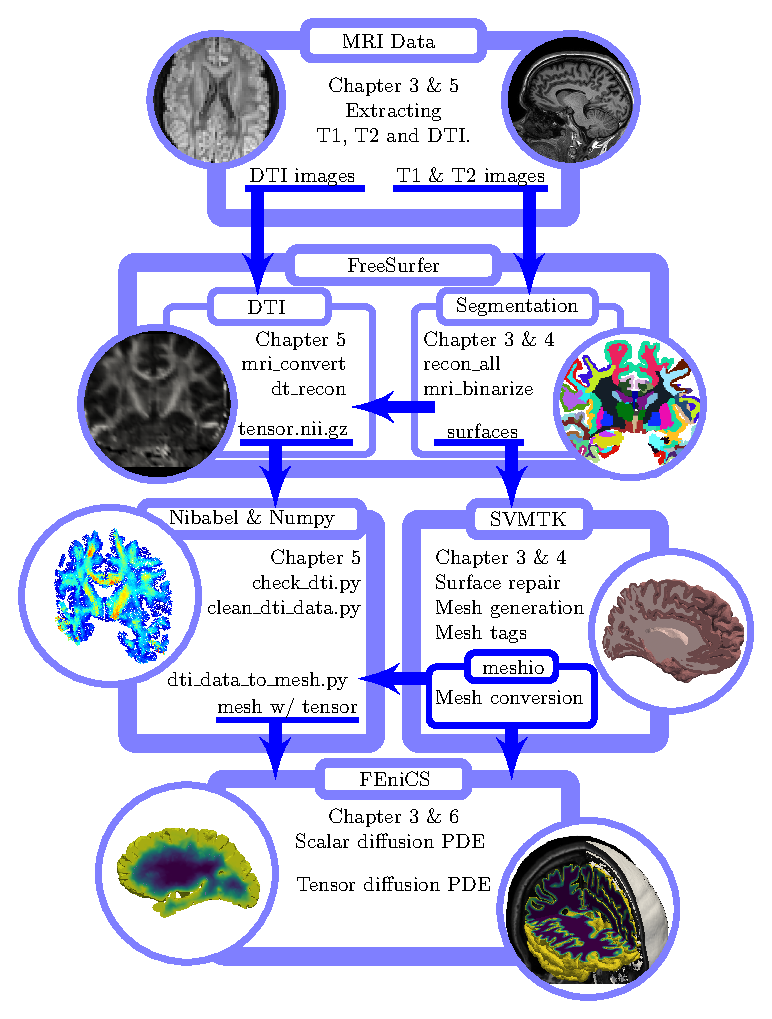
\includegraphics[width=0.95\textwidth]{./graphics/chp2/pipeline-overview.pdf} 
  \caption{Overview of the imaging, segmentation, meshing, simulation and 
visualization pipeline. T1, T2, and DTI images have already been discussed.  
Freesurfer and segmentation are discussed in 
Section~\ref{sec:chp2:tools:freesurfer}. Nibabel and Numpy are Python libraries; 
the former is used for neuroimaging applications and the latter is used 
primarily for the convenient manipulation of tensors. {\svmtk} is a 
computational geometry package, written for this book, which is specialized for 
creating brain meshes and {\fenics} is a Python library for high-performance 
finite element method computations.}
  \label{fig:chp2:imaging-pipeine-overview}
\end{figure}

\subsection{FreeSurfer for MRI processing and segmentation}
\label{sec:chp2:tools:freesurfer}
\index{FreeSurfer}
\index{segmentation}

FreeSurfer \cite{dale1999cortical} is an open source software suite
for the segmentation (identification of different brain regions), processing,
visualization, and analysis of human brain MR images. FreeSurfer is
well established, well documented, and widely used and we refer to the
FreeSurfer website for extensive documentation, online tutorials,
support, an overview of publications and general installation
instructions \cite{freesurfer}. Generally, all \freesurfer{} commands
also have extensive documentation available via \emp{-{}-help}.  At the time of 
writing, FreeSurfer provides step-by-step installation guides for 
Linux\footnote{\url{https://surfer.nmr.mgh.harvard.edu/fswiki//FS7\_linux}}
and Mac\footnote{\url{https://surfer.nmr.mgh.harvard.edu/fswiki//FS7\_mac}}.  
We will discuss the Linux installation process, here, for completeness. 

To install FreeSurfer on Ubuntu Linux, we suggest downloading the most
recent FreeSurfer tar archive\footnote{See for example \url{https://surfer.nmr.mgh.harvard.edu/fswiki/FS7\_linux}}
locally, for instance under \emp{/home/me/local/src}. If the name of this
file is \emp{freesurfer.tar.gz}, unpack the archive via
\ubuntu{\$ tar -zxvpf freesurfer.tar.gz}
\noindent The next step is to configure your environment for using
FreeSurfer. If your FreeSurfer archive has been unpacked at
\emp{/home/me/freesurfer}, then you can configure your FreeSurfer 
environment manually by adding the following lines
at the end of the file named \emp{.bashrc} in your home
directory:
\begin{lstlisting}[style=bashStyle]
export FREESURFER_HOME=/home/me/freesurfer 
export SUBJECTS_DIR=$FREESURFER_HOME/subjects 
source $FREESURFER_HOME/SetUpFreeSurfer.sh
\end{lstlisting}
  


\index{Freeview}
\noindent The {FreeSurfer} programming team requires that each user
acquire a license file to use the software; the license file is free,
and to acquire it, follow the registration directions at the FreeSurfer
website \cite{freesurfer}. Finally, FreeSurfer comes packaged
with the Freeview visualization tool. Test Freeview (and your
FreeSurfer installation) by opening a new terminal (noting the
FreeSurfer environment commands appearing on top), and typing
\terminal{\$ freeview \&}
\noindent to open the Freeview user interface.

We will use the command \emp{dt\_recon} in FreeSurfer, which has
additional requirements: tcsh\footnote{tcsh refers to a specific type of Unix 
shell.  A Unix shell is a command-line interpreter; there are many such shells 
used in a Unix environment (such as Ubuntu Linux).} and FSL. The installation 
of tcsh can be done from the terminal with the following command lines.
\ubuntu{\$ sudo apt update  \\
\$ sudo apt install tcsh}

FSL is a comprehensive library for functional MRI, MRI, and DTI brain imaging
data~\cite{jenkinson2012fsl}, and we refer the reader to its website for
installation
instructions\footnote{See https://fsl.fmrib.ox.ac.uk/fsl/fslwiki/FslInstallation.}. Note
that FSL, like FreeSurfer, requires a license to be operational.

\subsection{NiBabel: A python tool for MRI data}
\label{sec:chp2:tools:nibabel-numpy}

The Python module NiBabel~\cite{brett_matthew_2020_4295521} provides read and write
access to several neuroimaging file formats. The module is part of
NIPY, \footnote{See \url{https://nipy.org/}.} a community for neuroimaging
data analysis via Python. NiBabel can be installed using pip, for example, via the  
following terminal command:
\ubuntu{\$ sudo apt install python3-pip \\
\$ sudo pip3 install nibabel}
\noindent We will use Nibabel to work with image data in Python in 
Chapter~\ref{chp:chp4} and onwards.

\subsection{\svmtk{} for volume mesh generation}
\label{sec:chp2:tools:meshing:svmtk}
\index{SVM-Tk}

The Surface Volume Meshing Toolkit (\svmtk{}) is a toolkit for
generating meshes with subdomains based on surfaces and segmentations
provided by FreeSurfer. In particular, \svmtk{} provides a
Python-based interface to the Computational Geometry Algorithms
Library (CGAL)~\cite{fabri2000design} and provides tools for both
fixing and marking surfaces to enable a relatively robust mesh
generation for the various compartments of the brain.  We refer to the
\svmtk{} documentation\footnote{See https://github.com/SVMTK/SVMTK.} for
general installation instructions including a detailed list of
dependencies (including CGAL and a number of packages available
e.g.~through the Ubuntu package manager).

\subsection{The FEniCS Project for finite element simulation}
\label{sec:chp2:tools:fenics}
\index{FEniCS}
\index{FEniCS!tutorial}

We will use the open source FEniCS Project~\cite{alnaes2015fenics,
  logg2012automated} as our finite element software. FEniCS
includes both a C++ and a Python interface; we will use the Python
interface throughout. We refer to the FEniCS Project website for
extensive documentation, support, an overview of publications, and general
installation instructions \cite{fenicsproject}. In particular, we
strongly encourage the reader to become familiar with FEniCS and the finite
element method via the introductory FEniCS tutorial
\cite{langtangen2016solving}.

There are many ways to install the FEniCS Project software; including
the use of Docker images, using pre-built Anaconda packages, or from
source. Two simple ways of installing FEniCS are via Docker
images (see the FEniCS Project
website\footnote{\url{https://fenicsproject.org/download/}}) and via Ubuntu
package managers. For the latter, use the following terminal commands:
\terminal{%
\$ sudo apt-get install software-properties-common \\
\$ sudo add-apt-repository ppa:fenics-packages/fenics \\
\$ sudo apt-get update \\
\$ sudo apt-get install {\ddash}no-install-recommends fenics
} 


\subsection{ParaView and other visualization tools}
\label{sec:chp2:paraview}

\index{ParaView}
We recommend using ParaView~\cite{ahrens2005paraview} to visualize the 
simulation results, and other meshing objects, we will discuss throughout the 
book.  For installation instructions, see the
ParaView website\footnote{See \url{https://www.paraview.org/}.}. On Ubuntu
Linux, ParaView can be installed with the following
terminal command:
\ubuntu{\$ sudo apt-get install paraview}
\noindent After installation, ParaView can be launched with
\terminal{\$ paraview \&}

An optional but useful tool for visualizing surfaces (in the form
of surface STL files) is Gmsh~\cite{geuzaine2009gmsh}. For installation
instructions, see the Gmsh
website\footnote{See \url{http://gmsh.info/\#Download}.}. On Ubuntu Linux,
Gmsh can be installed with the following terminal command:

\ubuntu{\$ sudo apt-get install gmsh}


For quick plotting in Python, the Python package Matplotlib
is very convenient~\cite{hunter2007matplotlib}. The pyplot module of
Matplotlib can be imported in a Python script (as any other Python
module) as:
\begin{python}
import matplotlib.pyplot as plt
\end{python}

\subsection{Meshio for data and mesh conversion}
\label{sec:chp2:meshio}

\index{meshio}
We recommend using meshio \cite{schlomer2020nschloe} for conversion
between computational mesh formats. The meshio suite can convert
between various unstructured mesh formats, for instance between the
CGAL medit file format (.mesh) and the FEniCS mesh format (.xml or
.h5). To install meshio, the pip installer is
suggested, \footnote{See \url{https://pypi.org/project/meshio/}.} for example, via typing the following in the terminal:
\ubuntu{\$ sudo pip3 install meshio[all]}

\subsection{Testing the software pipeline}
\label{sec:chp2:tools:testing}

To verify that all software dependencies are correctly installed, we
provide a test script (in \emp{mri2fem/chp2}); the test script can 
be executed with the command
\terminal{\$ python3 test\_book\_software.py}
The script will check each software dependency and output a response indicating 
whether it is installed or not. 
If the software is not installed, the response is a detailed description of ways to correctly install it including links to installation guides: 
\terminal{Checking FEniCS installation.\\\\
\hspace*{1cm}	FEniCS is not installed\\
\hspace*{1cm}	Follow the installation guide at\\
\hspace*{1cm} 	https://fenicsproject.org/
}
If the software is installed, the response is a single-line response confirming that the software is installed:
\terminal{Checking FEniCS installation. => FEniCS installed}


